\chapter{Erstellung der Computerspielengines}
\label{chapter:erstellung-der-computerspielengines}

Nachdem Patchwork auf unterschiedlichste Aspekte analysiert und das Brettspiel als Computerprogramm umgesetzt wurde, werden nachfolgend die verschiedenen Computerspielengines für das Spiel implementiert.

\section{Ansatz A: Zufallsauswahl der Spielzüge}
\label{section:erstellung-ansatz-a}

Um eine Computerspielengine zu erstellen, muss das Trait \code{Player}, welcher in Codeausschnitt \ref{code:player-trait} zu sehen ist, von der Engine implementiert werden. Dafür müssen die zwei Methoden \code{name()} und \code{get\_action()}. Die erste Methode gibt den Namen der Computerspielengine zurück, um sie während des Spiels identifizieren zu können, während die zweite Methode die Aktion als \code{PlayerResult<Action>} zurückgibt, die der Spieler machen möchte und benötigt als Eingabe den aktuellen Zustand des Spiels.

\lstinputlisting[
    label={code:player-trait},
    caption={Definition des Player-Traits},
    captionpos=b,
    language=Rust,
    firstline=0,
]{res/code/player-trait.rs}

Die einfachste Computerspielengine ist der \code{RandomPlayer}, in Codeauschnitt \ref{code:random-player} zu sehen, welcher einen Spieler repräsentiert, der zufällige Züge macht. Zur Auswahl der Züge verwendet die Engine den Zufallsgenerator Xoshiro256++, der einen der möglichen Spielzüge im aktuellen Spielzustand \code{game} auswählt, die durch den Aufruf der Methode \code{game.get\_valid\_actions()} bereitgestellt werden. Diese Computergegner ist gut für Vergleichszwecke im späteren Kapitel \nameref{chapter:evaluation} geeignet, da die zufälligen Züge eine Baseline gegen die komplexeren, strategischen Entscheidungen der anderen Computerspielengines bildet.

\lstinputlisting[
    label={code:random-player},
    caption={Definition des RandomPlayers},
    captionpos=b,
    language=Rust,
    firstline=0,
]{res/code/random-player.rs}

\section{Ansatz B: Greedy-Algorithmus}

TODO: auch Evaluator

\pagebreak

\section{Ansatz C: Principal-Variation-Search}
\label{section:erstellung-ansatz-b}

Der dritte und erste richtige Versuch eines starken Computerspielgegners ist der \acl{PVS} Spieler. Für das Finden der besten Aktion verwenden der \acs{PVS} Spieler verwendet dabei eine optimierte Variante des Alpha-Beta-Suchalgorithmus, die \acf{PVS}. Bei der \ac{PVS} werden mehrere Änderungen vorgenommen. Zuerst wird der klassische Minimax-Algorithmus mittels Negamax implementiert. Bei Nullsummenspielen wie Patchwork ist der maximale Wert des einen Spielers immer der negierte minimale Wert des anderen Spielers ($\max\left(a,b\right) = -\min\left(-a,-b\right)$) \cite[S. 9]{2020.MinimaxTheorem}. Bei Negamax wird dies ausgenutzt, indem immer dieselbe Funktion aufgerufen wird und das Ergebnis negiert wird, anstatt zwei verschiedene Fälle für den min- und max-Spieler zu haben. Dies funktioniert aber nur, wenn der aktive Spieler nach jedem Spielzug wechselt. Dies ist in Patchwork nicht der Fall, kann in der Computerspielimplementierung aber erzwungen werden, indem der \code{do\_action} Methode ein \enquote{force player switch} Parameter übergeben wird. Würde der Spieler im Normalfall nicht wechseln, so wird einfach ein Spielerwechsel erzwungen und dem neuen Spieler nur die \emph{Phantom}-Aktion zur Verfügung gestellt. So kann auch die Suche in Patchwork ohne Probleme als Negamax implementiert werden, was die Implementierung vereinfacht.

Um genauer auf die weiteren Unterschiede von \ac{PVS} im Vergleich zur Alpha-Beta Suche eingehen zu können, müssen zuerst die in der Suche auftretenden Knotentypen erläutert werden:

\vspace*{-0.5cm}

\begin{figure}[!ht]
    \centering
    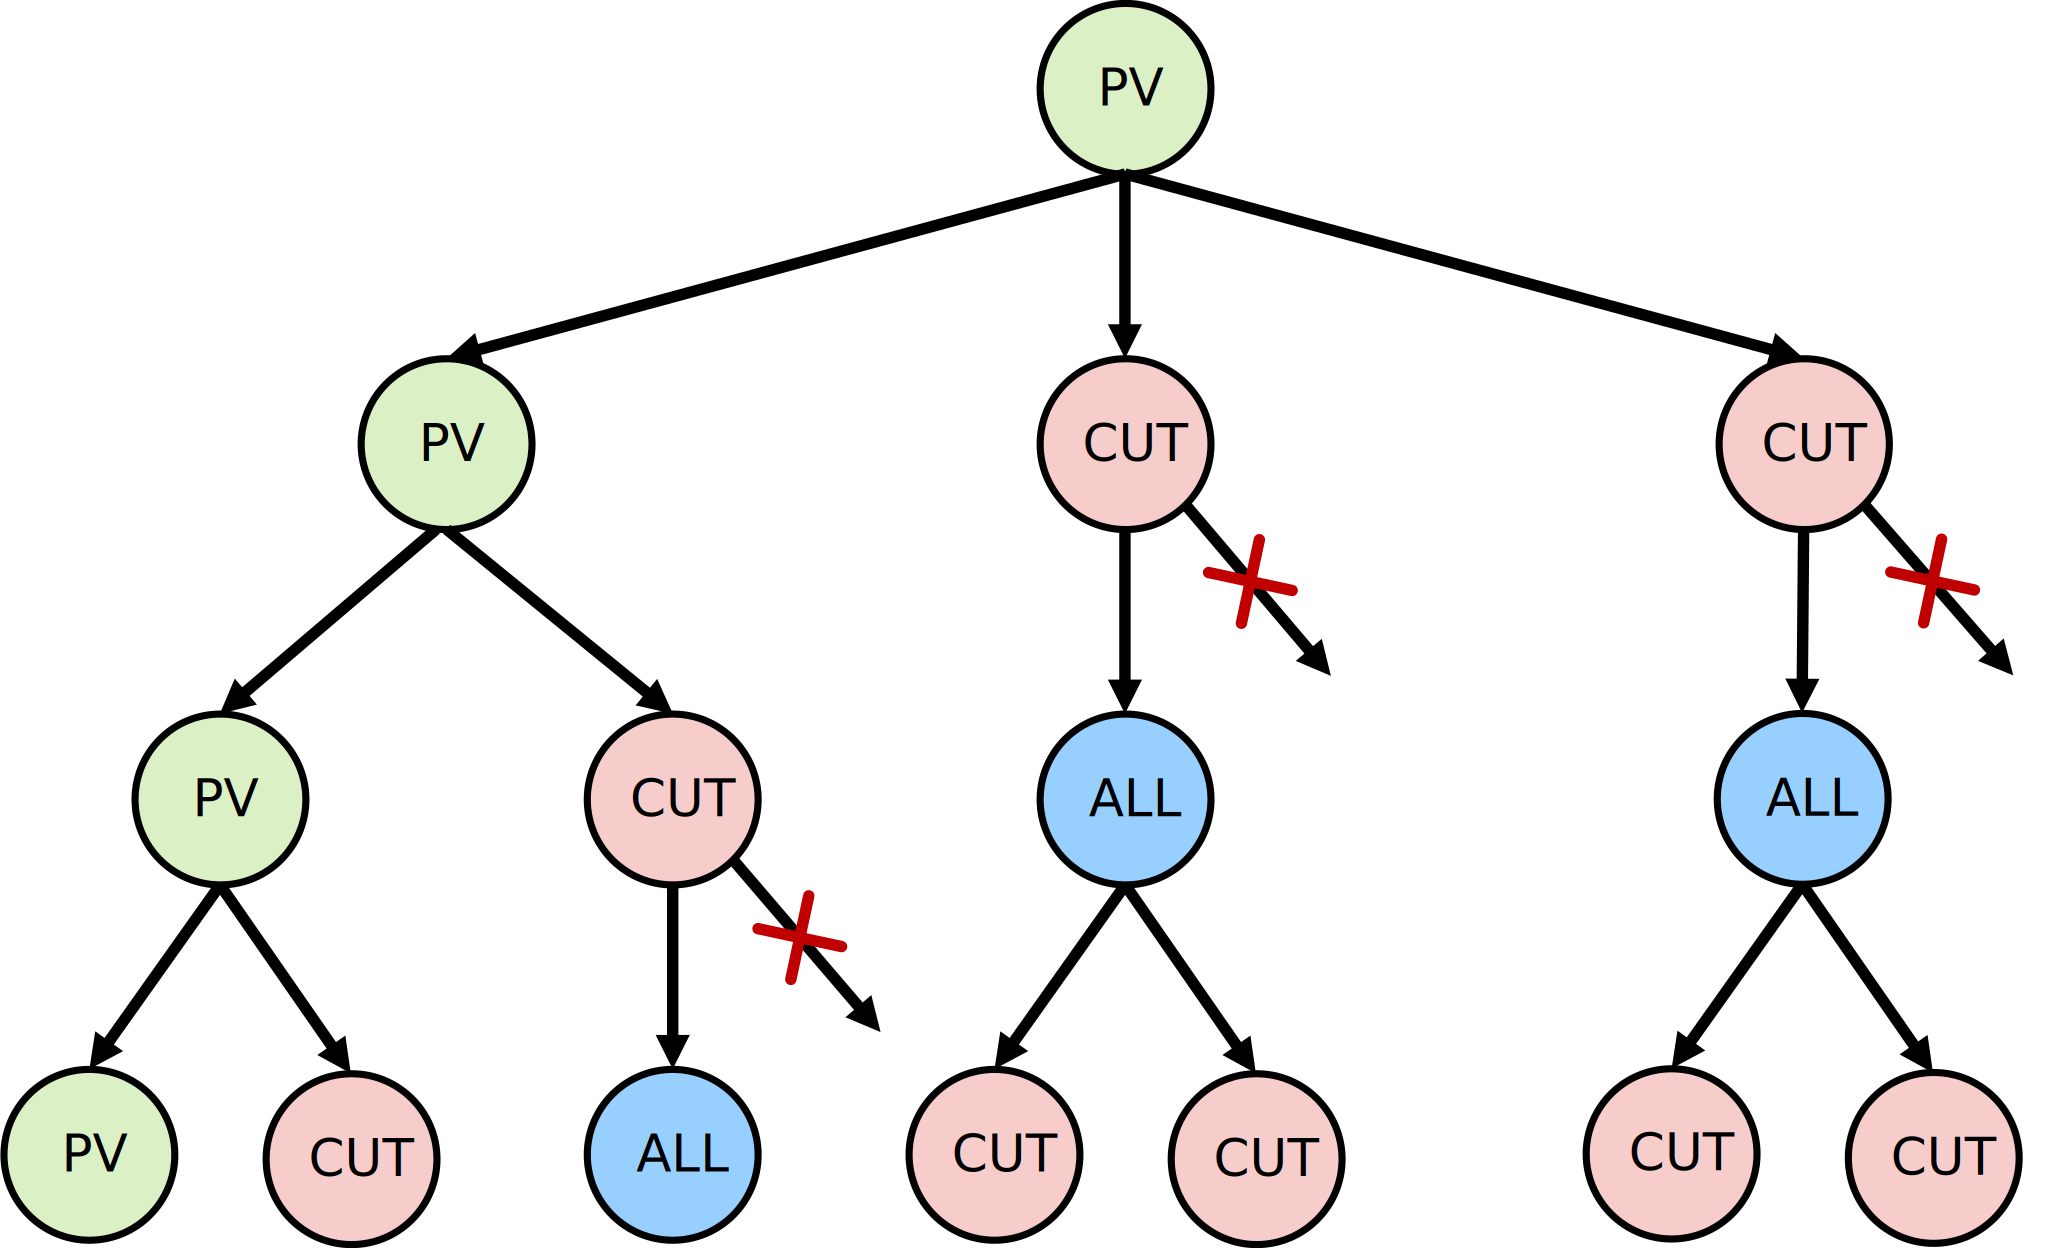
\includegraphics[width=0.75\textwidth]{res/pictures/minimal-search-tree.pdf}
    \caption{Minimaler Suchbaum bei der Alpha-Beta Suche}
    \label{fig:minimal-search-tree}
\end{figure}

\begin{itemize}
    \item \labeltext{\emph{\acs{PV}-Knoten}}{text:pv-node} oder \emph{Typ-1-Knoten}: Die \ac{PV} ist eine Sequenz an Aktionen, bei denen beide Spieler immer die für sich beste Aktion wählen. Es handelt es also um den \enquote{perfekten} Spielverlauf, bei dem kein Pruning stattfinden kann. \cite[S. 316f.]{2005.EnhancedForwardPruning}
    \item \vspace*{-0.125cm} \labeltext{\emph{Cut-Knoten}}{text:cut-node} oder \emph{Typ-2-Knoten}: Sind Knoten, bei denen ein $\beta$-Cutoff stattgefunden hat, \dash es gab eine Suche mit den Grenzen $\left[\alpha, \beta\right]$ und der Wert war $\ge \beta$. Somit wurde in diesem Teilbaum für einen Spieler eine Aktion gefunden, die zu gut war, sodass der andere Spieler vorher eine andere Aktion auswählen wird, damit das Spiel überhaupt nicht in den Zustand dieses Knotens kommen kann. \cite[S. 324]{1975.AlphaBeta}
    \item \vspace*{-0.125cm} \labeltext{\emph{All-Knoten}}{text:all-node} oder \emph{Typ-3-Knoten}: Während der Suche aller Kinderknoten wurde kein Spielzustand gefunden, der besser als ein anderer Spielzustand, welchen der aktuelle Spieler durch das Ausführen einer anderen Aktion in einem anderem Teil des Suchbaums erreichen konnte. Bei einer Suche mit Grenzen $\left[\alpha, \beta\right]$ war die Evaluation aller Kinderknoten also $\le \alpha$. \cite[S. 446]{1985.ParallelAlphaBeta}
\end{itemize}

\vspace*{-0.13cm}

Mithilfe dieser Knotentypen lässt sich der minimale für Alpha-Beta-Pruning benötigte Suchbaum aufstellen \cite[S. 8]{1991.SingleAgentGameTreeSearch}. Dieser ist in Abbildung \ref{fig:minimal-search-tree} visualisiert. Da Alpha-Beta als Tiefensuche agiert, werden immer zuerst alle \hyperref[text:pv-node]{\acs{PV} Aktionen / Knoten} durchsucht. Jeder \hyperref[text:pv-node]{\emph{\acs{PV}-Knoten}} hat dabei immer genau einen weiteren \hyperref[text:pv-node]{\emph{\acs{PV}-Knoten}} sowie mehrere \hyperref[text:cut-node]{\emph{Cut-Knoten}} als Kinder. Die \hyperref[text:cut-node]{\emph{Cut-Knoten}} erzeugen dabei einen Teilbaum, bei dem sich immer wieder \hyperref[text:cut-node]{\emph{Cut-Knoten}} und \hyperref[text:all-node]{\emph{All-Knoten}} abwechseln. Bei \hyperref[text:cut-node]{\emph{Cut-Knoten}} muss immer nur das erste Kind durchsucht werden, während bei allen anderen Kinderknoten ein $\beta$-Cutoff stattfinden kann. Bei \hyperref[text:all-node]{\emph{All-Knoten}} müssen immer alle Kinderknoten durchsucht werden.

\acl{PVS} setzt an dieser Stelle an, indem versucht wird den minimalen Suchbaum auch während der Suche zu erhalten. Dazu wird die Alpha-Beta-Suche mit einer iterativen Tiefensuche kombiniert, \dash zuerst wird der gesamte Suchbaum mit Tiefe 1 durchsucht, dann mit Tiefe 2 und so weiter. Dieser Vorgang wiederholt sich, bis die Suchzeit vorbei ist. In jeder Iteration, wird dabei in jeder Ebene die beste gefundene Aktion, die \acl{PV}, gespeichert. In der nächsten Iteration wird dann davon ausgegangen, dass es sich bei der \acl{PV} der vorherigen Suche auch weiterhin um die \acl{PV} handelt, auch wenn nun eine Ebene tiefer gesucht wird. Sollte dies der Fall sein, können sehr große Teilbereiche des Baums schnell geprunt werden. Die iterative \ac{PVS} Tiefensuche ist dabei durch die größere Anzahl an geprunten Knoten im Regelfall schneller als die Alpha-Beta Suche mit einer festen Tiefe \cite[S. 13]{2017.Minimax}.

\begingroup

\setlength{\textfloatsep}{0pt}
\setlength{\intextsep}{0pt}

\refstepcounter{lstlisting}
\addcontentsline{lol}{lstlisting}{\protect\numberline{\thelstlisting}Pseudocode vom Principal-Variation-Search Algorithmus}

\begin{algorithm}[!ht]
    \caption{Pseudocode vom Principal-Variation-Search Algorithmus}
    \label{algo:principal-varation-search}
    \begin{algorithmic}[1]
        \Function{pvs}{$game$,\, $\alpha$,\, $\beta$,\, $depth$}
        \If{$depth == 0$ oder $game$ ist Terminalzustand}
        \State \Return $color\ \cdot $ \Call{evaluation}{$game$} \Comment{$max$-Player $color = 1$, sonst $-1$}
        \EndIf
        \For{each valid $action$ of $game$}
        \State $game.$\Call{do\_action}{$action$}
        \If{$action$ ist erste Aktion} \Comment{$\acs{PV}$-Action}
        \State $value = -$\Call{pvs}{$game$,\, $-\beta$,\, $-\alpha$,\, $depth - 1$} \label{alg:pvs-line-8}
        \Else
        \State $value = -$\Call{pvs}{$game$,\, $-\alpha - 1$,\, $-\alpha$,\, $depth - 1$} \Comment{\small \acf{ZWS}} \label{alg:pvs-line-10}
        \If{$\alpha < value < \beta$}
        \State $value = -$\Call{pvs}{$game$,\, $-\beta$,\, $-\alpha$,\, $depth - 1$} \label{alg:pvs-line-12}
        \EndIf
        \EndIf
        \State $game.$\Call{undo\_action}{$action$}
        \If{$value \ge \beta$}
        \State \Return $\beta$ \Comment{$\beta$-Cutoff}
        \EndIf
        \State $\alpha = \max\left(\alpha, value\right)$ \label{alg:pvs-line-19}
        \EndFor
        \EndFunction
    \end{algorithmic}
\end{algorithm}

\endgroup

In Pseudocode \ref{algo:principal-varation-search} ist die \ac{PVS}-Suche abgebildet. Alle Aktionen werden bei jeden Methodenaufruf so angeordnet, dass die \acl{PV} der vorherigen Suche die erste Aktion ist. Da dort ein \hyperref[text:pv-node]{\emph{\acs{PV}-Knoten}} erwartet wird, findet eine Suche mit dem normalen $\alpha$-$\beta$-Fenster statt (\hyperref[alg:pvs-line-8]{Zeile 8}). In allen anderen Fällen soll so schnell wie möglich bewiesen werden, dass man sich nicht mehr in einem \hyperref[text:pv-node]{\emph{\acs{PV}-Knoten}} befindet. Dazu wird die untere Begrenzung des $\alpha$-$\beta$-Fensters auf die Evaluation gesetzt (\hyperref[alg:pvs-line-19]{Zeile 19}). Handelt es sich bei der ersten Aktion tatsächlich um die \acl{PV}, so müssten alle weiteren Aktionen schlechter sein und somit eine Evaluation $\le \alpha$ zurückgeben. Um dies so schnell wie möglich zu beweisen, wird eine \acf{ZWS}, eine Suche mit einem Fenster $\left[\alpha, \alpha + 1\right]$, ausgeführt (\hyperref[alg:pvs-line-10]{Zeile 10}) \cite[S. 317]{2005.EnhancedForwardPruning}. Dadurch, dass die obere Grenze mit $\alpha + 1$ so niedrig wie möglich ist, werden deutlich mehr $\beta$-Cutoffs produziert als mit dem normalen $\beta$ Parameter. Solange der tatsächliche Wert auch unterhalb von $\alpha$ liegt, stellt das kein Problem dar. Ist diese Annahme falsch, so muss die Suche mit dem normalen $\alpha$-$\beta$-Fenster erneut durchgeführt werden, um die tatsächliche Evaluation des Knotens zu erhalten (\hyperref[alg:pvs-line-12]{Zeile 12}) \cite{2002.PrincipalVariationSearch}. Ist die tatsächliche Evaluation besser als der derzeitige $\alpha$-Wert, so war auch die Annahme, dass die erste Aktion die \acl{PV} ist falsch und der Knoten wird als die neue \acl{PV} festgesetzt (\hyperref[alg:pvs-line-19]{Zeile 19}) \cite[S. 5]{1999.SolutionTreesGameTreeSearch}.

\vspace*{-5cm}

\pagebreak

Die gesamte Implementation des \ac{PVS}-Algorithmus zusammen mit allen nachfolgend vorgestellten Modifikationen ist in Anhang \ref{code:pvs-search} zu finden.

\subsection{Aktionen-Anordnung}

TODO:
\cite{2022.MoveOrdering}
Anordnung nicht Sortieren -> Warum überhaupt anordnen und warum nicht sortieren?
-> insertion sort??
Wie gemacht? -> Table mit linearer Interpolation based timeboard position
heatmap generierung erläutern
heatmaps erläutern und warum sinnvoll erscheint
müsste eigentlich symmetrisch sein

\begin{figure}[!ht]
    \centering
    \begin{minipage}{.11\textwidth}
        \centering
        \includegraphics[width=\linewidth]{res/pictures/assets/17-front.png}
    \end{minipage}
    \begin{minipage}{.78\textwidth}
        \centering
        \includegraphics[width=\linewidth]{res/pictures/plots/17-action-ordering.pdf}
    \end{minipage}
    \begin{minipage}{.11\textwidth}
        \hfill
    \end{minipage}
    \captionof{figure}{Heatmap des Flicken 17}
    \label{fig:action-ordering-patch-17}
\end{figure}

\begin{figure}[!ht]
    \centering
    \begin{minipage}{.11\textwidth}
        \centering
        \includegraphics[width=0.667\linewidth]{res/pictures/assets/21-front.png}
    \end{minipage}
    \begin{minipage}{.78\textwidth}
        \centering
        \includegraphics[width=\linewidth]{res/pictures/plots/21-action-ordering.pdf}
    \end{minipage}
    \begin{minipage}{.11\textwidth}
        \hfill
    \end{minipage}
    \captionof{figure}{Heatmap des Flicken 21}
    \label{fig:action-ordering-patch-21}
\end{figure}

\begin{figure}[!ht]
    \centering
    \begin{minipage}{.78\textwidth}
        \centering
        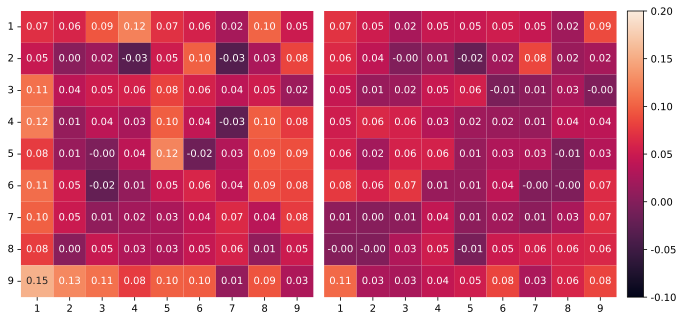
\includegraphics[width=\linewidth]{res/pictures/plots/special-action-ordering.pdf}
    \end{minipage}
    \captionof{figure}{Heatmap des Spezialflicken}
    \label{fig:action-ordering-special-patch}
\end{figure}

TODO:

\subsection{Transposition Table und Zobrist Hashing}

TODO:

\subsection{Aspiration Windows}

Eine mögliche Verbesserung der Iterativen Tiefensuche liegt in der Verwendung von Aspiration Windows. Bei der einfachen Implementierung der Tiefensuche ist der initiale Aufruf der \ac{PVS}-Suche immer mit $\alpha = -\infty$ und $\beta = \infty$. Bei Aspiration Windows wird diese Annahme insofern aufgelockert, indem davon ausgegangen wird, dass sich der Wert der nächsten Suchiteration nicht viel von dem Wert der vorherigen Suche unterscheidet. Deshalb wird statt dem gesamten Bereich nur ein Fenster (Aspiration Window) der Größe $\Delta$ um den vorherigen Suchwert erkundet. \cite{2003.AspirationWindows}

Da das initiale Fenster deutlich schmaler ist, können während der Suche im Normalfall mehr $\beta$-Cutoffs erreicht werden, was somit gleichzeitig einer kürzeren Suche entspricht. In den meisten Fällen gibt die Suche mit dem Aspriation Window auch wieder einen Wert innerhalb des Fensters von $\alpha$ und $\beta$ zurück. Ist dies nicht der Fall, muss die Suche zwingend erneut mit einem breiterem Aspiration Window wiederholt werden, was ein Nachteil bei der Verwendung ist.

\refstepcounter{lstlisting}
\addcontentsline{lol}{lstlisting}{\protect\numberline{\thelstlisting}Pseudocode: Aspiration Windows}

\begin{algorithm}[!ht]
    \caption{Pseudocode: Iterative Tiefensuche mit Aspiration Windows}
    \label{algo:aspiration-window}
    \begin{algorithmic}[1]
        \Function{search}{$game$}
        \State $\alpha \gets $ Starting-$\alpha$,\ \ $\beta \gets $ Starting-$\beta$,\ \ $\Delta \gets $ Starting-$\Delta$
        \For{$depth \coloneq 0$ bis Maximaltiefe}
        \State $value \gets \Call{principal\_variation\_search}{$\alpha$,\,$game$,\,$\beta$}$
        \If{Suchzeit vorbei}
        \State \textbf{break}
        \ElsIf{$value \le \alpha$} \Comment{Aspriation Window Fail-Low}
        \State $\alpha = value - \Delta$
        \State $\beta = (\alpha + \beta) / 2$ \Comment{$\beta$ in die Mitte des Fenster}
        \State $\Delta = \sfrac{4}{3}\cdot \Delta$
        \State \textbf{continue}
        \ElsIf{$value \ge \beta$} \Comment{Aspriation Window Fail-High}
        \State $\beta = value + \Delta$
        \State $\Delta = \sfrac{4}{3}\cdot \Delta$
        \State \textbf{continue}
        \EndIf
        \State $\Delta = $ \Call{new\_delta}{$value$,\, Starting-$\Delta$}
        \State $\alpha = value - \Delta$
        \State $\beta = value + \Delta$
        \EndFor
        \EndFunction
    \end{algorithmic}
\end{algorithm}

Wird ein Wert unterhalb von $\alpha$ zurückgegeben, handelt es sich um einen \emph{Fail-Low}, ist der Wert oberhalb von $\beta$, ist es ein \emph{Fail-High} Fall. Um im solch einen Failing-Fall möglichst effizient zu agieren, wird das Aspiration Window oftmals mit einem exponentiellen Backoff breiter gemacht, bis der Wert der Suche innerhalb des Fensters liegt. Die im Pseudocode \ref{algo:aspiration-window} verwendeten Werte für die Anpassung von $\alpha$, $\beta$ und $\Delta$ entsprechen dabei den Werten, welche in Stockfish verwendet werden, was eine der besten Schach-Computerspielengines ist \cite{2024.StockfishBackoff} \cite{2024.Stockfish}. Aus diesem Grund verwendet der \ac{PVS}-Spieler den gleichen exponentiellen Backoff.

Bei einer einfachen Mimimax-Suche lässt sich in einem Fail-Fail die Fenstergrenze, welche nicht fehlgeschlagen ist, immer auf die andere Grenze setzten. Kommt es also zu einem Fail-High bei der Suche mit Aspiration Window $\left[\alpha, \beta\right]$, so könnte die nächste Suche mit $\left[\beta, \beta + \Delta\right]$ stattfinden. Bei der Suche des \ac{PVS}-Spielers ist dies aufgrund von Suchinstabilität nicht der Fall. Suchinstabilität heißt, dass eine wiederholte Suche eines Spielzustands nicht immer die gleiche Evaluation zurückgeben muss \cite{2003.SearchInstability}. Diese Suchinstabilität kann bereits durch die Verwendung der gespeicherten Evaluationen aus der Transposition Table entstehen \cite{2003.SearchInstability}. Im Falle der Aspiration Windows bedeutet dies, dass eine Suche, die vorher mit Fail-High abgebrochen wurde, in der darauffolgenden Suche einen Fail-Low erzeugen kann. Deshalb wird der Wert von $\beta$ im Pseudocode zum Beispiel nur in die Mitte des Fensters verschoben.

\subsection{Suchselektivität}

Shannon führt in seinem Wert \emph{\enquote{Programming a Computer for Playing Chess}} eine Klassifizierung der Suchmethoden in einem Spielbaum ein, die zwei Haupttypen umfasst: \textbf{Typ-A} ist eine vollständige Brute-Force-Suche durch den gesamten Baum bis zu einer gewissen Tiefe \cite[S. 8]{1950.ChessShannon}. Bei der \textbf{Typ-B} werden die Äste des Spielbaums so selektiv ausgewählt, dass interessante Teilbäume tiefer durchsucht werden und uninteressante Teilbäume nur reduziert oder gar nicht durchsucht werden.

Im Bereich der Sucherweiterungen werden in Schach normalerweise Aktionen wie das Schlagen von Schachfiguren oder Schachsetzten berücksichtigt \cite[S. 14]{1950.ChessShannon}\cite{2023.StockfishTerminology}\cite{2002.SearchExtensions}. Während solche Aktionen in Patchwork nicht existieren, gibt es zwei Ereignisse, die für einen Spieler besonders interessant sind: Das Erhalten des $7\times 7$ Sonderplättchens sowie das Legen eines Spezialflicken. Bei beiden Aktionen wird die Suche deshalb um eine Tiefenebene erhöht (Anhang \ref{code:pvs-search-extension}). Im Fall der Null-Fenster-Suche werden keine Sucherweiterungen angewendet.

Für Patchwork sind Suchreduktionen im Bereich der Typ-B-Suche jedoch von größerer Bedeutung. Um bei Spielzuständen, die viele Aktionen erlauben und somit einen hohen Verzweigungsfaktor haben, den Suchaufwand möglichst minimal zu halten, sollte ein großer Teil der Aktionen nur reduziert durchsucht oder ganz weggelassen werden. Im \ac{PVS}-Spieler kommen hierzu zwei Konzepte zum Einsatz: \ac{LMR} und \ac{LMP}.

Bei einer Suche mit einigermaßen guter Zugreihenfolge tritt ein \hyperref[text:beta-cutoff]{\emph{Beta-Cutoff}} wenn überhaupt normalerweise am ersten \hyperref[text:pv-node]{\emph{\acs{PV}-Knoten}} auf \cite{2007.LMR}. Deswegen werden bei \ac{LMR} nur die ersten Aktionen mit der vollen Tiefe durchsucht und alle weiteren Aktionen werden insofern nichts interessantes passiert mit einer reduzierten Tiefe durchsucht. Als Nachteil muss aber bei einem zu guten Ergebnis über $\alpha$ der Teilbaum mit voller Tiefe erneut durchsucht werden \cite{2007.LMR}. Im \ac{PVS}-Spieler wird die Suche bei allen nicht \ac{PV}-Aktionen ab einer gewissen Tiefe auf ein Drittel der originalen Tiefe reduziert. Vorher wird die Suche immer um eine Ebene reduziert.

Bei \ac{LMP} wird ein noch drastischere Ansatz verfolgt, indem bestimmte Teilbäume gar nicht mehr anstatt nur reduziert durchsucht werden \cite{2023.StockfishTerminology}. Dabei handelt es sich um einen Tradeoff zwischen Suchgenauigkeit bzw. -stabilität und Zeit. Je mehr Aktionen \emph{geprunt}, also weggelassen werden, desto tiefer kommt die Suche. Gleichzeitig könnten aber so Teilbäume übersehen werden, welche einen besseren Spielverlauf beinhalten. Um die sehr große Anzahl an Aktionen, die bei einem Spielzustand auftreten können (1345) zu reduzieren, werden sehr viele Aktionen im \ac{PVS}-Spieler geprunt. Während in der ersten Ebene immer alle Aktionen betrachtet werden, wird in den späteren Tiefen immer nur sichergestellt, dass mindestens 3 Platzierungsmöglichkeiten für jeden Flicken überprüft werden. Die Auswahl dieser Aktionen basiert dabei auf der Bewertung der Aktionen-Anordnung. Die spezifischen Pruning-Werte wurden ermittelt, indem verschiedene Konfigurationen für die Starttiefe und die Anzahl an Platzierungsmöglichkeiten pro Flicken mit dem klassischen Alpha-Beta-Minimax-Algorithmus (wie in \ref{algo:minimax-alpha-beta}) gegeneinander spielten. Dabei wurden die besten Werte für den \ac{PVS}-Spieler übernommen.

\subsection{Lazy-SMP}

Der bisher beschriebene \ac{PVS}-Spieler läuft Single-Threaded ab. Da heutige Computer mehrere Kerne besitzen, sollten diese aber auch verwendet werden. Für Mimimax sowie davon abgeleitete Algorithmen existiert dazu eine einfache aber gleichzeitig effektive Parallelisierungsmöglichkeit.

Bei Lazy \ac{SMP}, werden $n$ parallele unabhängige Suchen gleichzeitig gestartet, welche sich nur die Transposition Table teilen. Dadurch, dass alle bereits durchsuchten Spielzustände in die Transposition Table eingefügt werden, wird sichergestellt, dass Spielzustände, welche zuvor von Threads erkundet wurden, nicht erneut durchsucht werden müssen.

TODO:

\section{Ansatz D: Monte Carlo Tree Search}
\label{section:erstellung-ansatz-c}

TODO:

\begin{itemize}
    \item Normaler MCTS
    \item UCT (Upper Confidence Bound for Trees)
    \item Parallel (Root und Leaf)
    \item Tree Reuse
    \item Evaluator (WinLoss, Score) -> In Eval genauer betrachten
\end{itemize}

\section{Ansatz E: AlphaZero}
\label{section:erstellung-ansatz-d}

TODO:

\begin{itemize}
    \item Änderungen Gegenüber MCTS / Generelle Funktionsweise
    \item Kodierung des Spielzustandes
    \item Netzwerk-Architektur
    \item Parallelization with Virtual Loss
    \item Training-Loop
\end{itemize}

\subsubsection*{Kodierung des Spielzustandes}

\begin{figure}[!ht]
    \centering
    \vspace*{-1.75cm}
    \includegraphics[width=\textwidth]{res/pictures/patch-zero-state.pdf}
    \caption{Zustandskodierung von PatchZero}
    \label{fig:patch-zero-state}
\end{figure}

TODO: LSTM Bild

\pagebreak

\subsubsection*{Netzwerk-Architektur}

\cite{2018.Lc0AlphaZero}
\cite{2019.SqueezeandExcitation}
\cite{2020.Lc0NetworkTopology}

\begin{figure}[!ht]
    \centering
    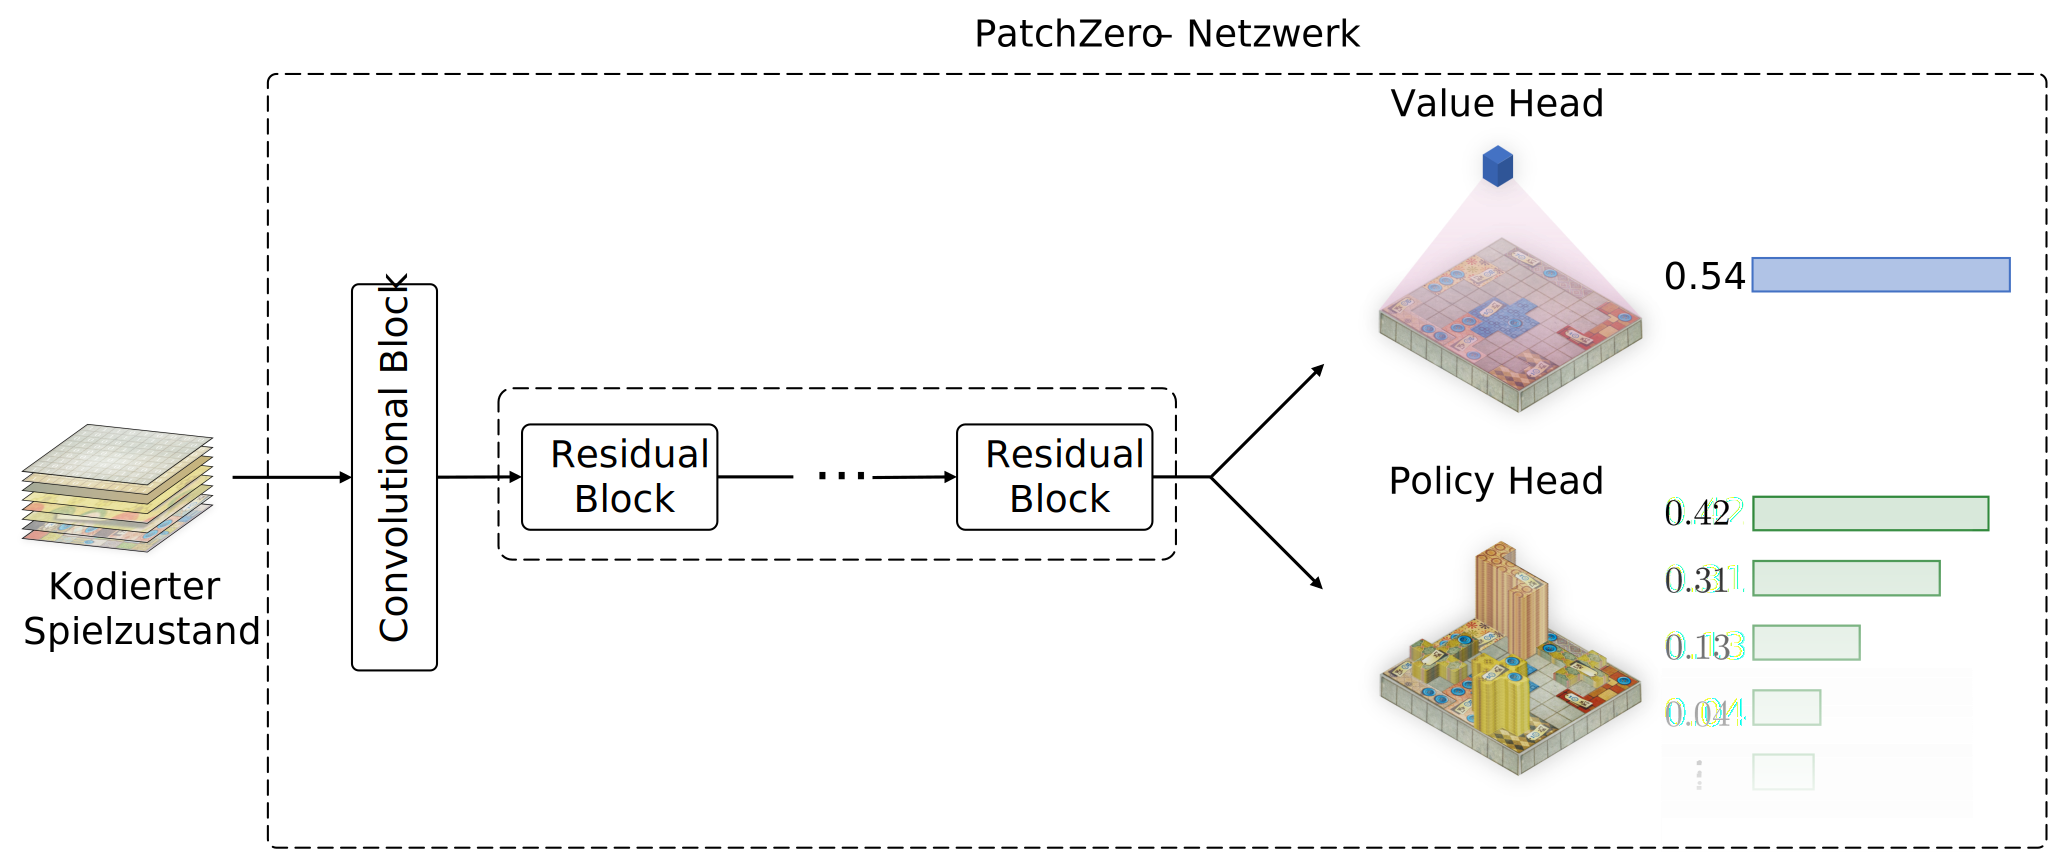
\includegraphics[width=\textwidth]{res/pictures/patch-zero-architecture.pdf}
    \caption{Architektur von PatchZero}
    \label{fig:patch-zero-architecture}
\end{figure}

TODO:

\begin{wrapfigure}{r}{0.25\textwidth}
    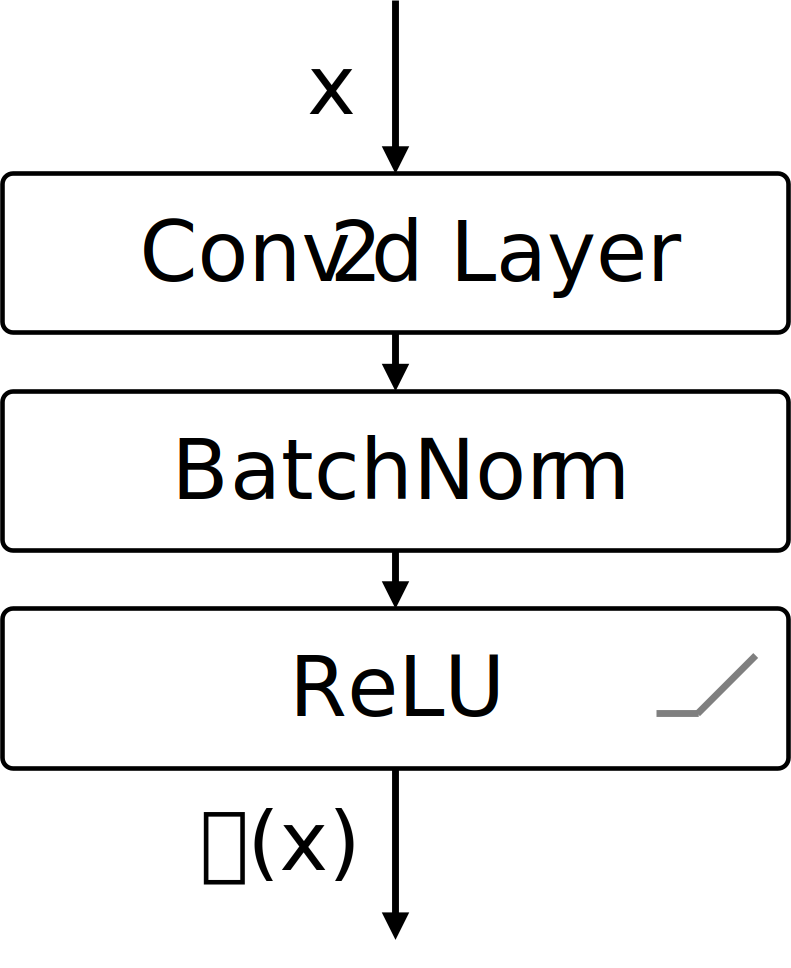
\includegraphics[width=0.2\textwidth]{res/pictures/conv-block.pdf}
    % \vspace{-10pt}
    % Das folgende ist ein Trick, um "Abbilgung x.y" in eine
    % eigene Zeile zu packen. Der Text zwischen [ und ] steht
    % im Abbildungsverzeichnis. Der Text darunter wird
    % tatsächlich angezeigt.
    \centering
    \caption[Convolutional Block]{\unskip}
    Convolutional Block
    \label{fig:conv-block}
\end{wrapfigure}

TODO:

\begin{wrapfigure}{l}{0.3\textwidth}
    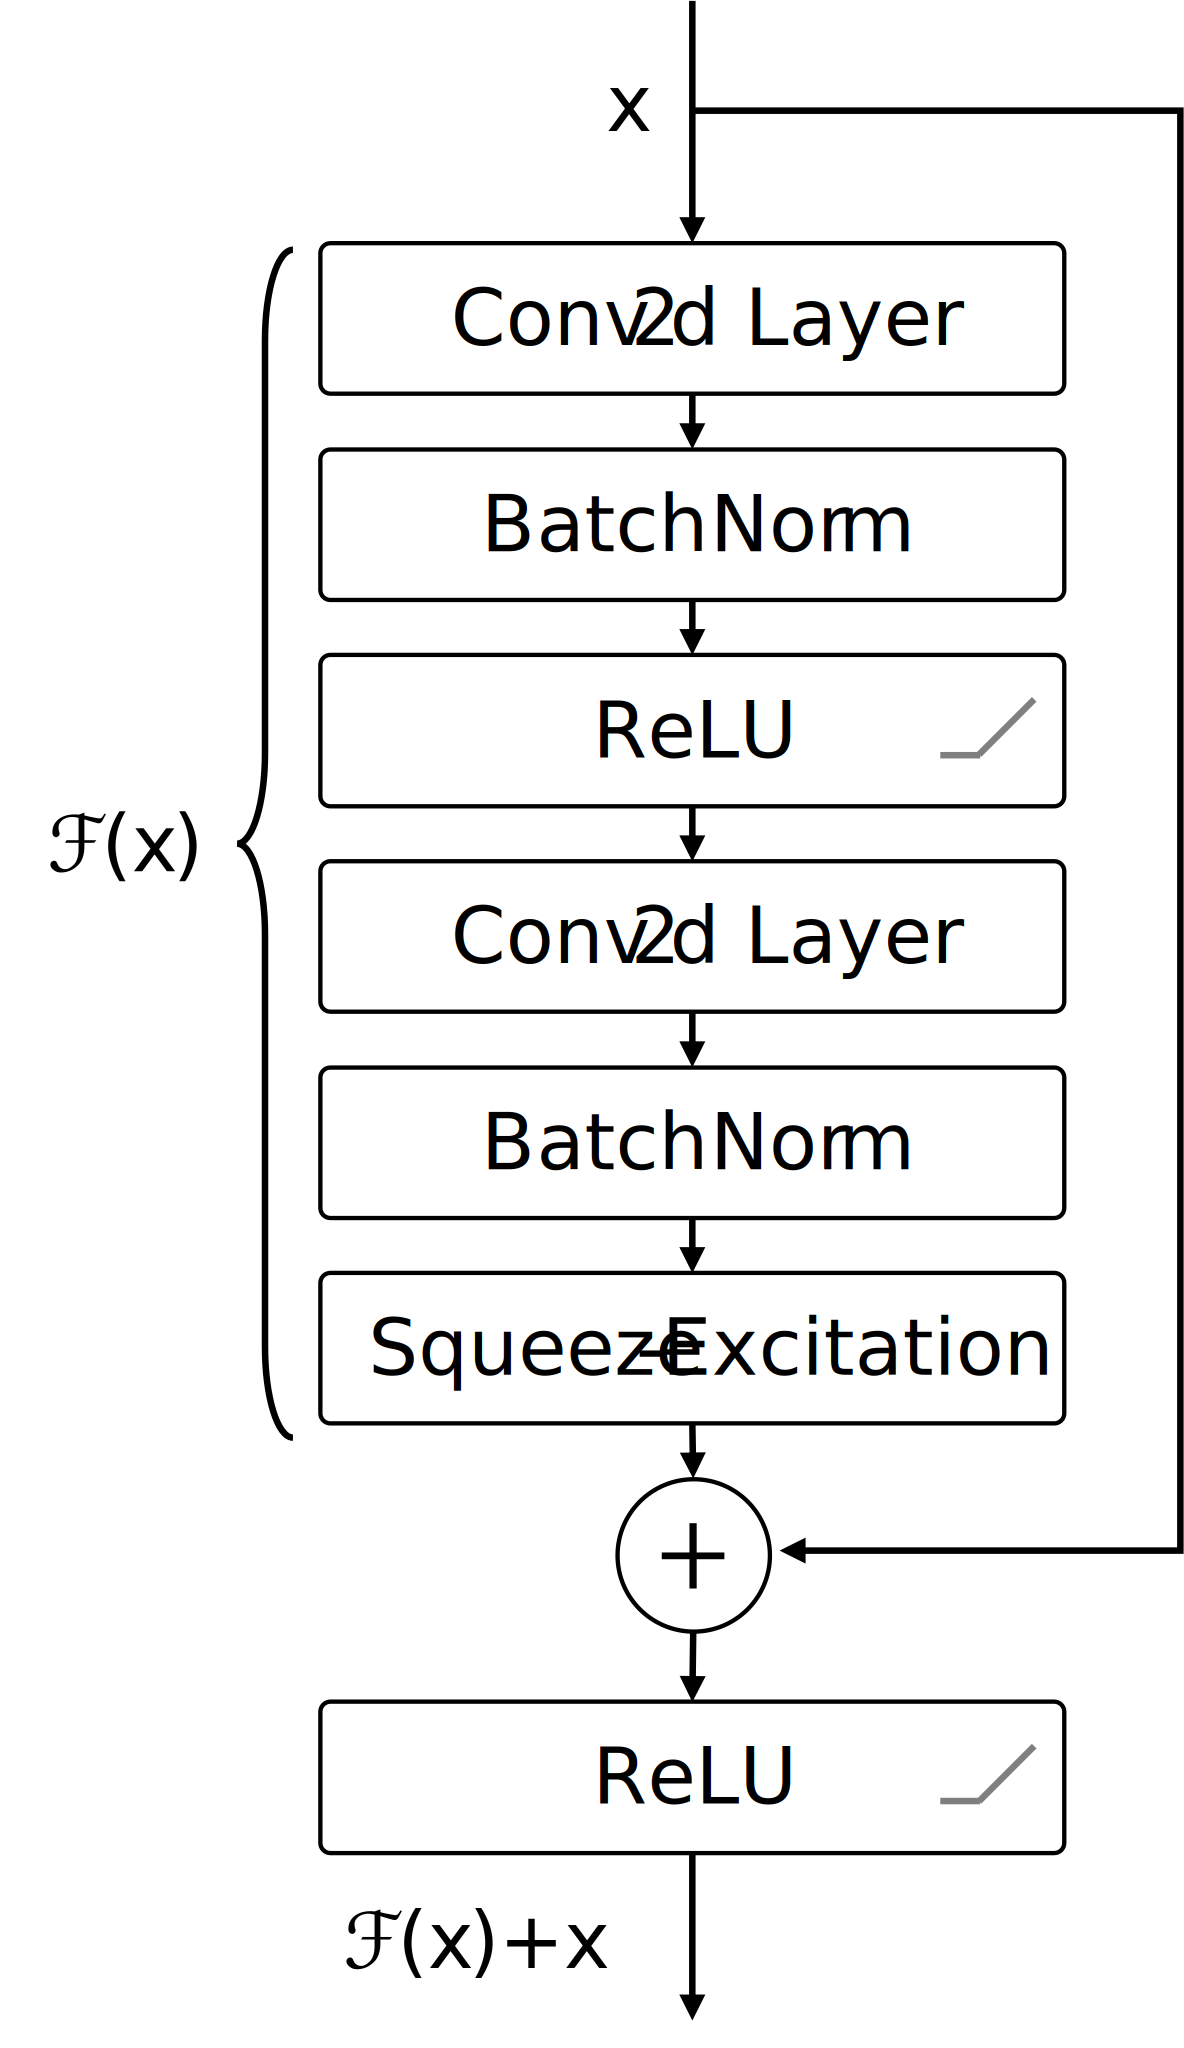
\includegraphics[width=0.25\textwidth]{res/pictures/res-block.pdf}
    % \vspace{-10pt}
    % Das folgende ist ein Trick, um "Abbilgung x.y" in eine
    % eigene Zeile zu packen. Der Text zwischen [ und ] steht
    % im Abbildungsverzeichnis. Der Text darunter wird
    % tatsächlich angezeigt.
    \centering
    \caption[Residual Block]{\unskip}
    Residual Block
    \label{fig:resblock}
\end{wrapfigure}

TODO:

\begin{wrapfigure}{r}{0.35\textwidth}
    \centering
    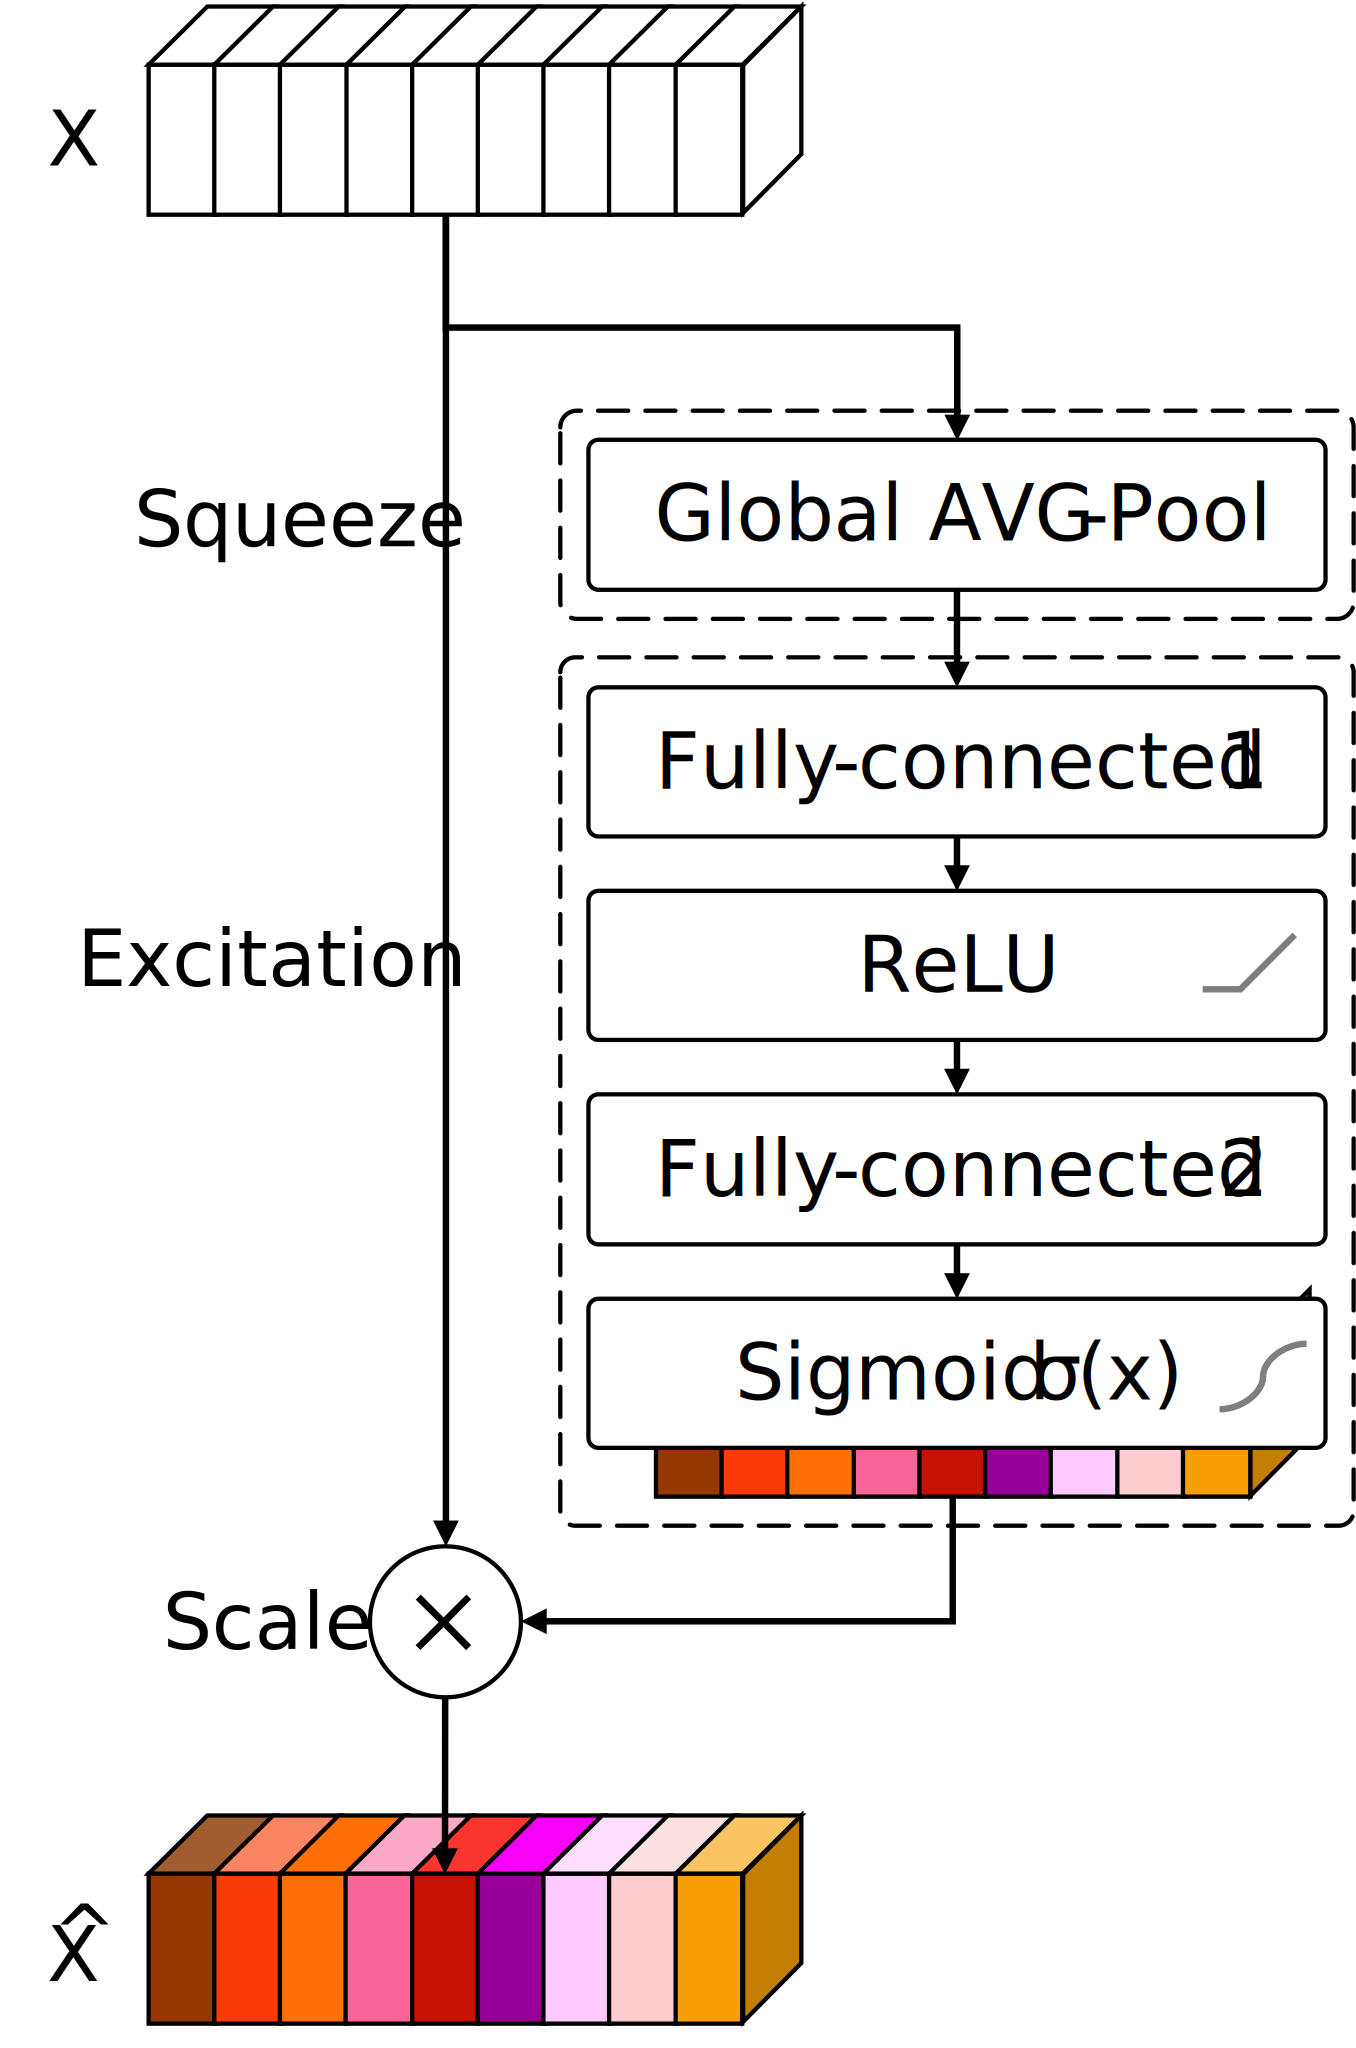
\includegraphics[width=0.3\textwidth]{res/pictures/squeeze-and-excitation-block.pdf}
    % \vspace{-10pt}
    % Das folgende ist ein Trick, um "Abbilgung x.y" in eine
    % eigene Zeile zu packen. Der Text zwischen [ und ] steht
    % im Abbildungsverzeichnis. Der Text darunter wird
    % tatsächlich angezeigt.
    \caption[Squeeze \& Excitation Block]{\unskip}
    Squeeze \& Excitation Block
    \label{fig:squeeze-and-excitation-block}
\end{wrapfigure}

TODO:

\pagebreak

\begin{figure}[!ht]
    \centering
    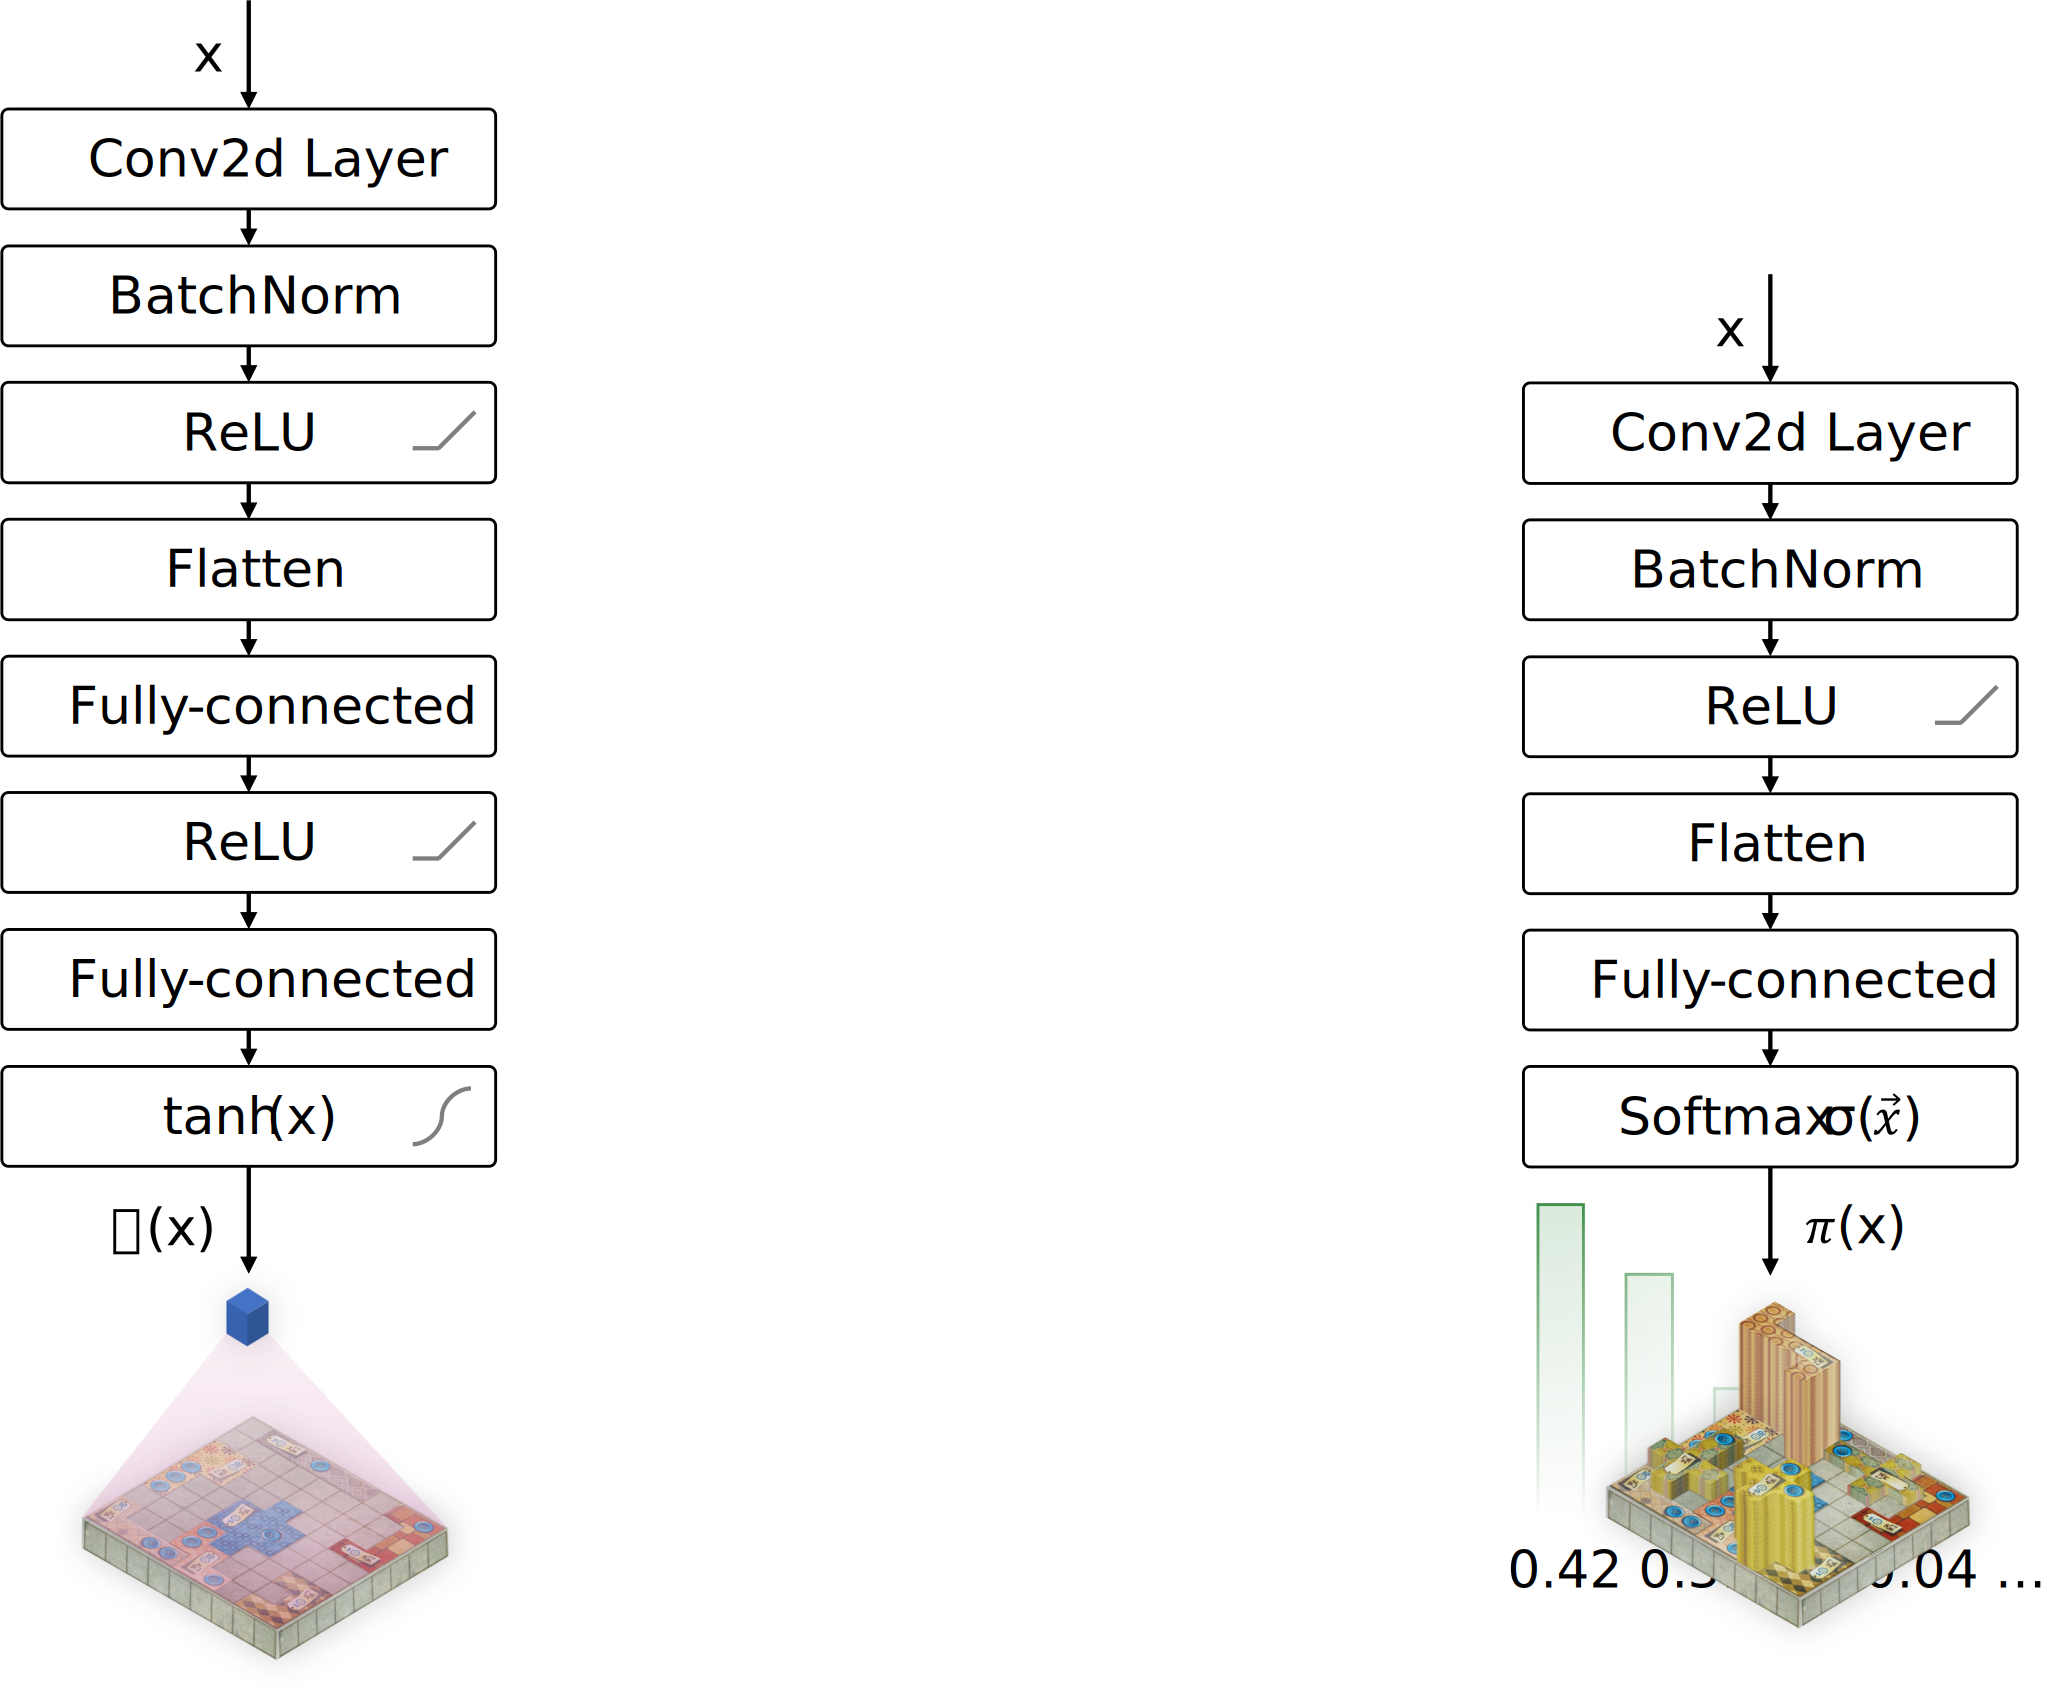
\includegraphics[width=0.7\textwidth]{res/pictures/value-and-policy-head.pdf}
    \\
    \begin{minipage}{.49\textwidth}
        \centering
        \captionof{figure}[Value Head von PatchZero]{\unskip}
        Value Head von PatchZero
        \label{fig:value-head}
    \end{minipage}
    \hfill
    \begin{minipage}{.49\textwidth}
        \centering
        \captionof{figure}[Policy Head von PatchZero]{\unskip}
        Policy Head von PatchZero
        \label{fig:policy-head}
    \end{minipage}
\end{figure}

TODO: